\documentclass{chi-ext}
% Please be sure that you have the dependencies (i.e., additional LaTeX packages) to compile this example.
% See http://personales.upv.es/luileito/chiext/

%% EXAMPLE BEGIN -- HOW TO OVERRIDE THE DEFAULT COPYRIGHT STRIP -- (July 22, 2013 - Paul Baumann)
% \copyrightinfo{Permission to make digital or hard copies of all or part of this work for personal or classroom use is granted without fee provided that copies are not made or distributed for profit or commercial advantage and that copies bear this notice and the full citation on the first page. Copyrights for components of this work owned by others than ACM must be honored. Abstracting with credit is permitted. To copy otherwise, or republish, to post on servers or to redistribute to lists, requires prior specific permission and/or a fee. Request permissions from permissions@acm.org. \\
% {\emph{CHI'14}}, April 26--May 1, 2014, Toronto, Canada. \\
% Copyright \copyright~2014 ACM ISBN/14/04...\$15.00. \\
% DOI string from ACM form confirmation}
%% EXAMPLE END -- HOW TO OVERRIDE THE DEFAULT COPYRIGHT STRIP -- (July 22, 2013 - Paul Baumann)

%\title{CHI \LaTeX\ Ext. Abstracts Template}
\title{Mute Robot - Cooperative Gameplay Through Body Language Communication}

\numberofauthors{6}
% Notice how author names are alternately typesetted to appear ordered in 2-column format;
% i.e., the first 4 autors on the first column and the other 4 auhors on the second column.
% Actually, it's up to you to strictly adhere to this author notation.
\author{
  \alignauthor{
  	\textbf{First Author}\\
  	\affaddr{AuthorCo, Inc.}\\
  	\affaddr{123 Author Ave.}\\
  	\affaddr{Authortown, PA 54321 USA}\\
  	\email{author1@anotherco.com}
  }\alignauthor{
  	\textbf{Fourth Author}\\
  	\affaddr{AuthorCo, Inc.}\\
  	\affaddr{123 Author Ave.}\\
  	\affaddr{Authortown, PA 54321 USA}\\
  	\email{author5@anotherco.com}
  }
  \vfil
  \alignauthor{
  	\textbf{Second Author}\\
  	\affaddr{AuthorCo, Inc.}\\
  	\affaddr{123 Author Ave.}\\
  	\affaddr{Authortown, PA 54321 USA}\\
  	\email{author2@anotherco.com}
  }\alignauthor{
  	\textbf{Fifth Author}\\
  	\affaddr{AuthorCo, Inc.}\\
  	\affaddr{123 Author Ave.}\\
  	\affaddr{Authortown, PA 54321 USA}\\
  	\email{author6@anotherco.com}
  }
  \vfil
  \alignauthor{
  	\textbf{Third Author}\\
  	\affaddr{AuthorCo, Inc.}\\
  	\affaddr{123 Author Ave.}\\
  	\affaddr{Authortown, PA 54321 USA}\\
  	\email{author3@anotherco.com}
  }\alignauthor{
  	\textbf{Sixth Author}\\
  	\affaddr{AuthorCo, Inc.}\\
  	\affaddr{123 Author Ave.}\\
  	\affaddr{Authortown, PA 54321 USA}\\
  	\email{author7@anotherco.com}
  }
}

% Paper metadata (use plain text, for PDF inclusion and later re-using, if desired)
\def\plaintitle{CHI LaTeX Extended Abstracts Template}
\def\plainauthor{Luis A. Leiva}
\def\plainkeywords{Game; Video games; Game design; Body language; Kinect}
\def\plaingeneralterms{Documentation, Standardization}

\hypersetup{
  % Your metadata go here
  pdftitle={\plaintitle},
  pdfauthor={\plainauthor},  
  pdfkeywords={\plainkeywords},
  pdfsubject={\plaingeneralterms},
  % Quick access to color overriding:
  %citecolor=black,
  %linkcolor=black,
  %menucolor=black,
  %urlcolor=black,
}

\usepackage{graphicx}   % for EPS use the graphics package instead
\usepackage{balance}    % useful for balancing the last columns
\usepackage{bibspacing} % save vertical space in references


\begin{document}

\maketitle

\begin{abstract}
Speech ability, a general habit becoming nature for us, plays an important role in our daily life, but if one day we can't speak anymore, using body language becomes a evident feasible way to communicate between human beings.
Mute Robot Game has been designed to provide players a new environment where they become a robot without speech ability. The game intend to supply players facing in challenging stages. 
Players communicate with body language, with an emphasis on cooperation to facilitate immersion with each other.
%Players need to cooperate with each other to pass challenges by using body language communication.
\end{abstract}

%\begin{abstract}
%In this sample we describe the formatting requirements for various %SIGCHI related submissions 
%and offer recommendations on writing for the worldwide SIGCHI %readership. 
%%Do not change the page size or page settings.
%Please review this document even if you have submitted to SIGCHI %conferences before, 
%some format details have changed relative to previous years.
%\end{abstract}

%[Section] Author Keywords
\keywords{\plainkeywords}
%\textcolor{red}{Mandatory section to be included in your final version.}

%[Section] ACM Classification Keywords
\category{K.8.0}{Personal Computing}{General \it{Games}}. 
%See \cite{ACMCCS} 
%See: \url{http://www.acm.org/about/class/1998/} 
%for help using the ACM Classification system.
%\textcolor{red}{Mandatory section to be included in your final version.}

%[Section] General Terms
%\terms{\plaingeneralterms}
%\textcolor{red}{Optional section to be included in your final version.}

% =============================================================================
\section{Introduction}
% =============================================================================

I'm BaoZi! I'm awesome!!!


% =============================================================================
\section{Design and Development}
% =============================================================================
Mute Robot is a cooperative puzzle platformer game using Unity3D engine\cite{Unity3D}. In our game, two players are in different rooms and connected by network. In each room, we provide a wii controller and a Kinect\cite{Kinect} device. wii\cite{Wii} controller is used to control the avator movement,like jump or move. in the mean time, Kinect is capturing player’s body language and apply the posture to the avator. With this setting, players cant talk to their teammate directly and the only way to communicate is using  their body language.


%why use wii, why not use pure Kinect control!?



\section{Using Body Language}
% =============================================================================
%關卡設計方式
In order to apply a new communication interface for user, Mute Robot is designed by using body language to communicate between players. Testing shows that using body language is an intuitive choice for player to communicate without speech ability.

\begin{figure}
  \centering
  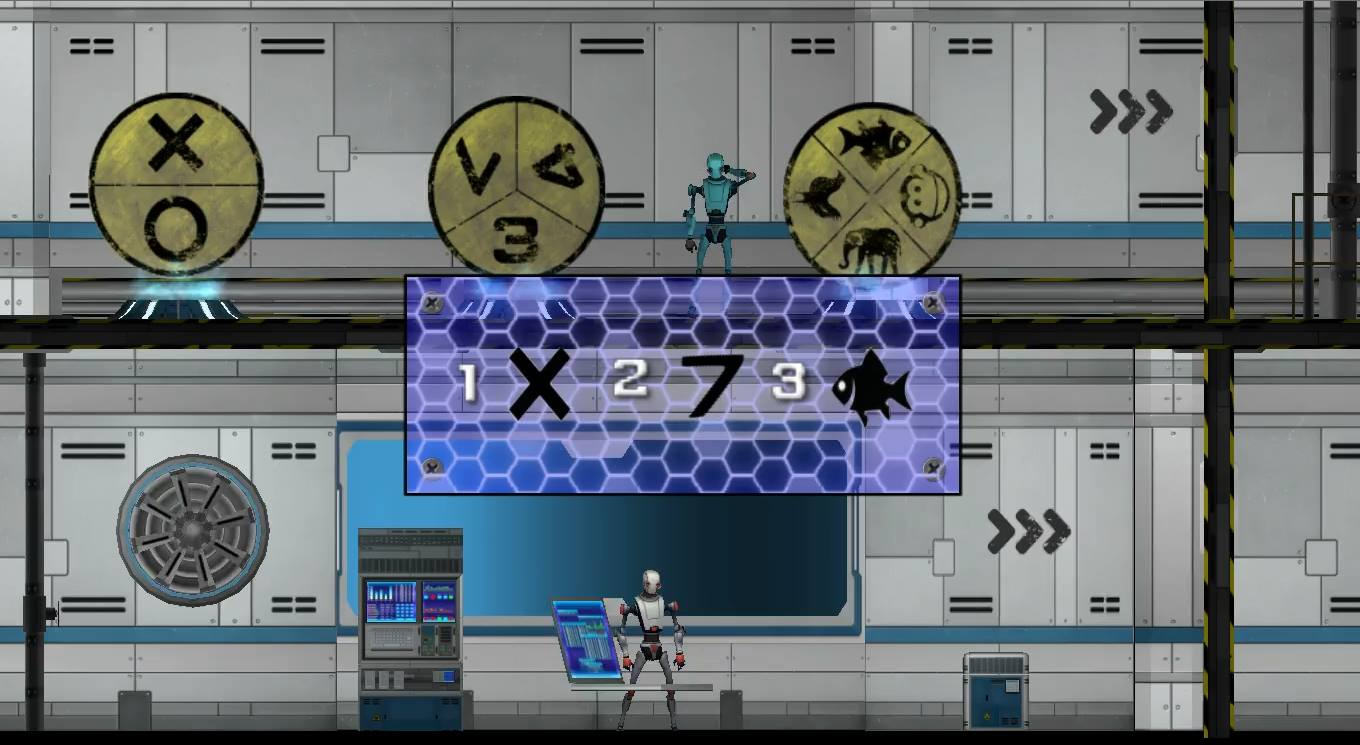
\includegraphics[width=\linewidth]{figures/Figure1.jpg}
  \caption{asymmetric puzzle system example}
  \label{fig:Figure1}
\end{figure}

To encourage players using body language, we design an asymmetric puzzle system, providing one player to receiving puzzle hints, and another player solving the puzzle. Take one of our game stage for example(fig. 1), there is a locked door on the right side which obstruct both players route to the next stage. With a view to opening the locked door, the underside player will receive some puzzle-solving message. The upper side player can't see the puzzle-solving hints but he can turn the wheel to the match puzzle answer. The only way to pass the stage needs two players' cooperation and communication with body language. As a result, the right side locked door will be opened when all wheels be turned to the right direction.

%If human beings lose speech ability, with no doubt, an intuition way for people communication is using body language. Based on past historical experience, using body language is a human instinct. In addition,  We assume that 

% =============================================================================
\section{Testing and Evaluation}
% =============================================================================
We recruited 16 participants without knowing each other, and randomly divided them into 8 groups, preparing camera and screen-captured software to attain playing information. 
On average, the total game duration is about 10 to 20 minutes. 
At the end of the game, we provided a questionnaire to invest the player experience and feedback.

\begin{figure}
  \centering
  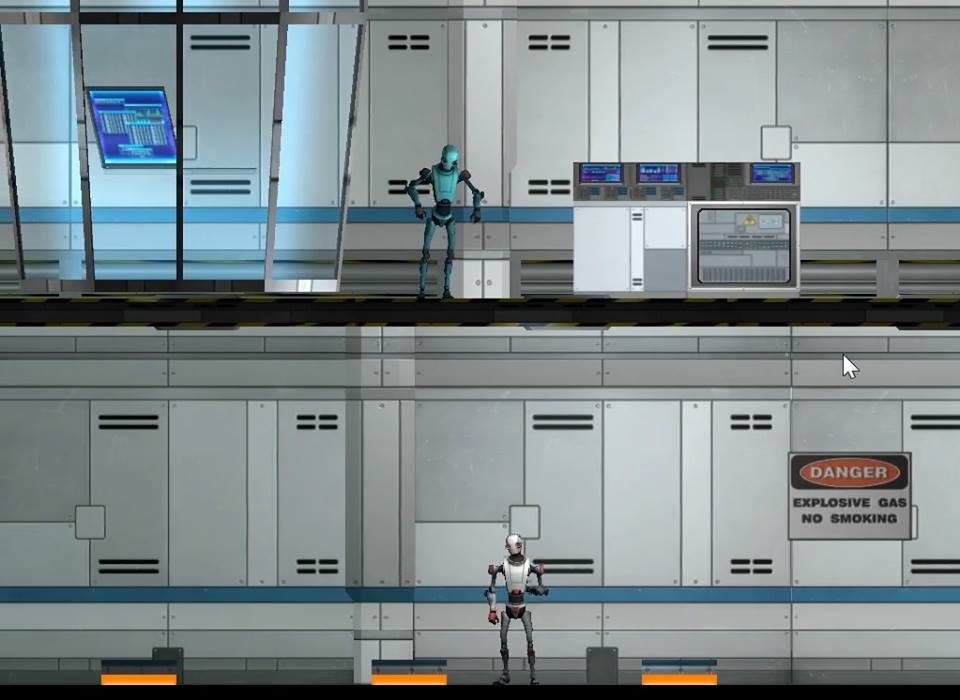
\includegraphics[width=0.8\linewidth]{figures/Figure2.jpg}
  \caption{emulate with body language}
  \label{fig:Figure2}
\end{figure}

Among player's playing experience, we find out some unique condition between players' body language communication: 
(1) Command style: player who receives puzzle-solving hint messages will command another player to do some action directly. For instance, player would wave his hand to tell another player to go back; or player likes to jump in place in order to imply another player to tread on the relaive position.
(2) Do by your own: player who receives puzzle-solving hint messages will do the puzzle-solving actions one time for another player to observe and emulate. For example, one of our game stage need to open the locked door by jumping on three buttoms respectively with different order(fig. 2).
(3) Pictogram style: player would use his own body to express what he see from puzzle-solving hint messages. For instance(fig. 3), one participant want to express letter ``N'', and her solution is using pictogram with body language to show the answer for another player.

\marginpar{
\begin{figure}
  \centering
  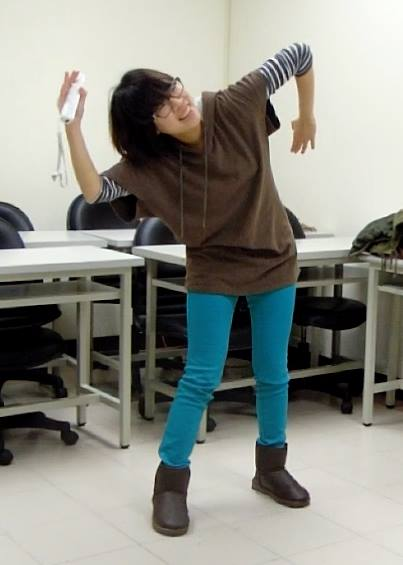
\includegraphics[width=0.8\linewidth]{figures/Figure3.jpg}
  \caption{player perform pictogram with body language}
  \label{fig:Figure3}
\end{figure}
}

\begin{figure}
  \centering
  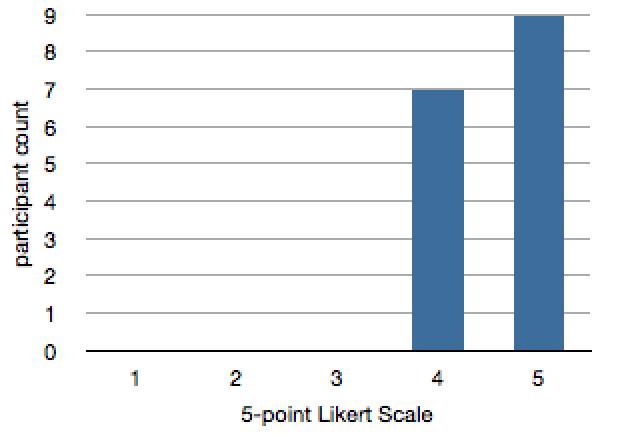
\includegraphics[width=0.8\linewidth]{figures/1_BLisInteresting.png}
  \caption{using body language is interesting}
  \label{fig:1_BLisInteresting}
\end{figure}

After we analyze statistics from the questionnare. we find some truth which can support our Mute Robot game design. 
Figure 4 shows out that all participants think using body language to communicate in puzzle game is interesting.
%有趣,了解對方的語言、有好感
Figure 5 shows that two-thirds players feel they can figure out another player's body language.


\begin{figure}
  \centering
  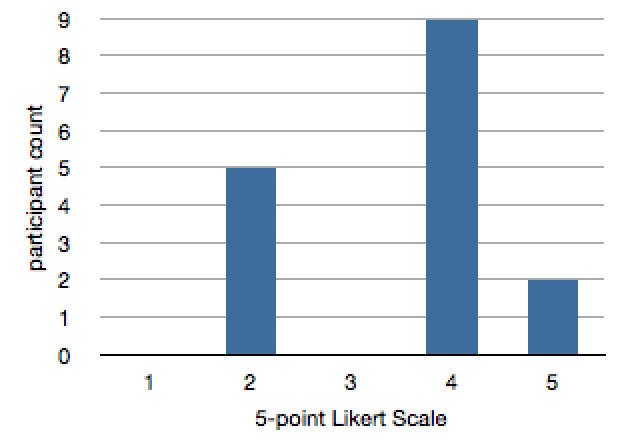
\includegraphics[width=0.9\linewidth]{figures/2_BLunderstand.png}
  \caption{is easy to figure out teammate's body language}
  \label{fig:2_BLunderstand}
\end{figure}

%\begin{figure}
%  \centering
%  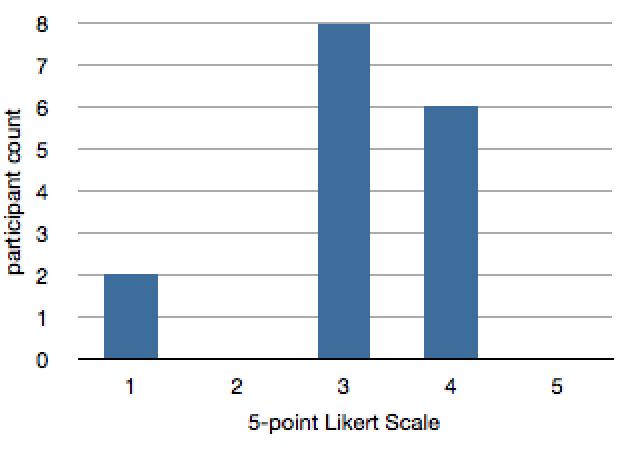
\includegraphics[width=0.8\linewidth]{figures/3_BLPositiveFeeling.png}
%  \caption{333}
%  \label{fig:3_BLPositiveFeeling}
%\end{figure}

%situations
%1. 命令句:如果畫面鐘有那個東西,會直接用指的, 回來手勢,
%2. 做給他看(踩左右中)
%3. 象行(angry中的N), 模仿動物 directly

%找16位玩家,不認識對方
%遊戲長度約10~20分鐘
%- # 
%- Body Language Communication (observation)
%- Satisaction Survey



% =============================================================================
\section{Future Work}
% =============================================================================

As we know, Kinect allow personal computer to track the gesture of our body as we move around, but it hasn't had the fine detail of our gestures, and particular, it hasn't really understood our hand. If one day, the ability for Kinect can recognize our hand gesture and facial expression, we can communicate with body language more precisely. 

On the other hand, Mute Robot game design is using asymmetric puzzle system to let players cooperate with each other to break through the game stage. In the futre, if both players can receive part of puzzle-solving hints and exchange messages with body language, we believe that it will have more interaction between players and become more interesting.

%1. 可以抓到表情、手指
%2. 可以做更複雜的關卡
%now:一個人告訴另一個人,不是兩邊整合訊息 (a告訴b
%improve:上下皆有一些資料,共同完成 a purpose

% =============================================================================
\section{Conslusion}
% =============================================================================
Mute Robot shows a new integration between current gameplay style and body language, where the interaction between game and human body movement form a unprecedented innovative gameplay empiriment.
Our statistics results indicate that Mute Robot can proliferation of communication and interaction between players.
The Kinect-based manipulation can facilitate the body language interation and intrinsically motivate the player.
Mute Robot provide a path towards future exploration of this relatively unexplored field of game design with capacious development space.

%數據 feadback 喜歡 
%這樣的作法、遊戲是蠻有發展空間的
%是一個很適合在kinect上的發展遊戲


\section{Acknowledgements}
We thank advisor Mike Y. Chen and the faculty and staff of National Taiwan University.
We would also like to express our gratitude towards all playtesters who have helped us in our many iterations. 


\section{References format}
References must be the same font size as other body text.
% REFERENCES FORMAT
% References must be the same font size as other body text.

\balance
\bibliographystyle{acm-sigchi}
\bibliography{chi14SGC-MuteRobot}

\end{document}